\section{Functions}
The next type of relations in this chapter are functions.
As we will find, function relations some of the most fundamental to math -- so important that we've already used them in various parts of the book completely none the wiser.
In this section, we will give this vital idea a proper construction in the language of sets.

\subsection{Definition}
As usual, let's begin our investigation with a definition:
\begin{define} \label{def:function}
	Let $(f,X,Y)$ be an ordered triple such that $f\subseteq X\times Y$.
	The ordered triple is a function if and only if
	\begin{axiomlist}
		\item (Total) for every $x\in X$, there exists $y\in Y$ such that $(x,y)\in f$,
		\item (Functional) if $(x,y)\in f$ and $(x,z)\in f$ implies $y=z$.
	\end{axiomlist}
\end{define}

We usually denote $X$ and $Y$ to be the \textit{domain} and \textit{codomain} and $f$ as the \textit{graph}.\footnote{
	The \textit{graph} of a function in this sense is not the \textit{plot} of the function as you've seen in previous classes.
	Instead, the graph of the function is simply relation that connects inputs to outputs, sort of like a web.
	While these two concepts are inherently related when they both exist, we will be running into plenty of examples where functions don't have reasonable plot presentations.
	From now on, I will refer to the thing we draw as a plot to save some confusion.}
While the ordered triple definition is needed in the formal definition of a function, we typically identify the function $(f,X,Y)$ as $f:X\to Y$\footnote{
	This notation is read as \textit{$f$ is a function mapping elements in $X$ to $Y$}
	} and reference the function simply by the symbol for its graph.
Also, if $(x,y)\in f$, we typically denote this with the much cleaner notation $f(x)=y$.
We note that two functions are considered equal if and only if $(f,X,Y)$ and $(g,X,Y)$ are equivalent as sets (i.e. the sets in the triple are equivalent component wise).
This might be different from the notion of function equality that is taught in prior classes as our definition here requires not only graph equivalence but also equivalence of the domains and codomains to the function.
We often denote the set of all functions of the form $X \to Y$ as the set $Y^X$.

With the formal statement out of the way, let's translate these to more manageable form.
Given any arbitrary $f:X\to Y$ satisfying \cref{def:function}, let's see what the conditions impose on the relation $f$.
To say $f$ is \textit{total} means that every element in the domain, $X$, has an associated element in the codomain $Y$.
That means evaluation for every $x$ in $X$ has an associated output $f(x)$, which should correspond nicely any previous understands of functions.
To say $f$ \textit{functional} means that each element in the domain relates uniquely to an element in the codomain.
Another term often used for this property is the notion that $f$ is \textit{well-defined}.
Notice that no where in our definitions here did we require our function $f$ to map entirely onto our codomain $Y$.
$Y$ here simply represents the target for which elements of the domain are mapped to.
To examine which elements are mapped to in the codomain, we turn to the following definition:

\begin{define}
	We call $f(A)$ the \textbf{image of $f$ under $A\subseteq X$}  if and only if
	\begin{equation}
		f(A):=\{f(a) : a\in A\}.
	\end{equation}
\end{define}

This is a general definition for the elements mapped to bay a particular subset of the domain, we shall denote the image $f(X)$ as the \textit{range}.
Now, contrast this definition of range with our definition of a codomain.
While not every element in a function's codomain needs to be related to an element in the domain, every element in a function's range must be related to an element in its domain.
This idea can be visualized in \cref{fig:function}, where the arrows between elements show the structure of the function's graph.
Since the element $z$ is unrelated to any element in $X$, we conclude $z$ is not in the range of $f$.\footnote{We note that $f(X)\subseteq Y$ for any well-defined function.}

\begin{figure}
\centering
\resizebox{0.7\linewidth}{!}{
	\begin{tikzpicture}
		\filldraw[white] (-7,-3) rectangle (7,3);

		\draw (-3,0) ellipse (1.5 and 3) node[yshift=3.5cm] {$X$};

		\draw (3,0) ellipse (1.5 and 3) node[yshift=3.5cm] {$Y$};
		\draw (3,0.8) ellipse (1 and 1.9);
		\draw[thick, ->] (5.3,1.8) node[xshift=.8cm] {$f(X)$} -- (4.1,1.5);

		\node (u) at (-3,2) {\Large$u$};
		\node (v) at (-3,0) {\Large$v$};
		\node (w) at (-3,-2) {\Large$w$};

		\node (x) at (3,2) {\Large$x$};
		\node (y) at (3,0) {\Large$y$};
		\node (z) at (3,-2) {\Large$z$};

		\draw[thick,->] (u.east) -- (y.west);
		\draw[thick,->] (v.east) -- (y.west);
		\draw[thick,->] (w.east) -- (x.west);

		\draw (0,-4) node {$f:X\to Y$};

	\end{tikzpicture}}
	\caption{}
	\label{fig:function}
\end{figure}

\begin{remark}
	If we refer back to the definition of cartesian products, we introduced the notion of indexing which consists of uniquely assigning each element of an indexing set $I$ to another collection of sets $\mathcal C$.
	One can easily deduce that this is exactly the definition of a function $I \to \mathcal C$.
	For this reason, we can generalize this denote any function of the form $I \to C$ an $I$-indexing on $C$.
	Then if $f$ is such an $I$-indexing, we denote the $i$th element\footnote{Note, $I$ does not need to be the subset of the integers, or any set of numbers for that matter.} of $c_i \in C$ as $c_i:= f(i)$.
\end{remark}

\begin{define}
	We call $f^{-1}(B)$ the \textbf{preimage of $f$ under $B\subseteq Y$}, where
	\begin{equation}
		f^{-1}(B):=\{x\in X : f(x)\in B\}.
	\end{equation}
\end{define}

By this definition, $f^{-1}(B)$ is understood as the set of elements that are mapped into $B$\footnote{i
	Note: this operation \textit{is not} equivalent to the inverse of a function, while the notation looks the same.
	However, if the inverse of a function exists, the preimage is indeed the image of the inverse under the same set.
	(See \cref{exer:preimg-imgbi})
}
An illustration of the concept is provided in \cref{fig:preimage}.
Note that $f^{-1}(Y)=X$. I will leave this as an exercise for the reader to check understanding.

\begin{prop} \label{prop:preimgimg}
	Let $f:X \to Y$ be a function then
	\begin{enumerate}
		\item $U \subseteq f^{-1}(f(U))$ for any $U \subseteq X$,
		\item $f(f^{-1}(V)) \subseteq V$ for any $V \subseteq Y$,
	\end{enumerate}
\end{prop}
\begin{proof}
	For (1), suppose $x \in U$.
	Letting $y:=f(x)$, we have $y \in f(U)$.
	By definition of preimage, we have $x\in f^{-1}(f(U))$ since $x$ maps to $y$.
	Therefore, $U \subseteq f^{-1}(f(U))$

	For (2), see \cref{exer:imgpreimg}
\end{proof}


\begin{figure}
	\centering
	\resizebox{0.7\linewidth}{!}{
	\begin{tikzpicture}
		\filldraw[white] (-7,-3) rectangle (7,3);

		\draw (-3,0) ellipse (1.5 and 3) node[yshift=3.5cm] {$X$};

		\draw (3,0) ellipse (1.5 and 3) node[yshift=3.5cm] {$Y$};
		\draw (-3,0.8) ellipse (1 and 1.9);
		\draw[thick, ->] (-5.3,1.8) node[left] {$f(\{y\})$} -- (-4.1,1.5);

		\node (u) at (-3,2) {\Large$u$};
		\node (v) at (-3,0) {\Large$v$};
		\node (w) at (-3,-2) {\Large$w$};

		\node (x) at (3,2) {\Large$x$};
		\node (y) at (3,0) {\Large$y$};
		\node (z) at (3,-2) {\Large$z$};

		\draw[thick,->] (u.east) -- (y.west);
		\draw[thick,->] (v.east) -- (y.west);
		\draw[thick,->] (w.east) -- (z.west);

		\draw (0,-4) node {$f:X\to Y$};
	\end{tikzpicture}}

	 \caption{} \label{fig:preimage}
\end{figure}

We also have the following definition for a very specific preimage:
\begin{define}
	Let $f:X \to Y$ be any function.
	For any element $y \in Y$, we denote the preimage $f^{-1}(\{y\})$ as the \textit{fiber} of $y$.
\end{define}

A common abuse of notation is to take $f^{-1}(y):=f^{-1}(\{y\})$ to mean the fiber of $y$ over $f$.

Let's prove the following propositions to strengthen our understanding of these definitions.

\begin{prop} \label{prop:unique-empty-function}
	There exists a unique function $\varnothing \to Y$ for any set $Y$.
\end{prop}
\begin{proof}
	Let $f:\varnothing \to Y$ and $g:\varnothing \to Y$ be functions.
	The domains and codomains are clearly the same thus it remains to show the graphs are equivalent.
	By \cref{exer:product-empty}, we have $\varnothing \times Y = \varnothing$.
	However, since the only subset of $\varnothing$ is $\varnothing$, thus we conclude $f$ and $g$ must be the same relation.
\end{proof}

\begin{prop} \label{prop:codomain-non-empty}
	Let $f:X \to Y$ be a function, then $Y$ is non-empty if $X$ is non-empty
\end{prop}
\begin{proof}
	Let's prove the contrapositive of the statement.
	Thus let $f$ be a function and suppose $Y$ is empty. Then since $f$ is a function, for each $x\in X$, there exists $y\in \varnothing$ such that $f(x)=y$.
	Since $y\in \varnothing$ is always false by definition of the empty set, for every $x$, the statement $x\in X$ must be false thus $X$ must be the empty set.
\end{proof}

\subsection{Compositions and Inverses}
\begin{define} \label{def:one-to-one-func}
	Let $f: X\to Y$ be a function. $f$ is said to be \textit{one-to-one (injective)} if for every $x_1,x_2\in X$ such that $f(x_1)=f(x_2)$ implies $x_1=x_2$ or equivalently, $x_1\neq x_2$ implies $f(x_1)\neq f(x_2)$.
\end{define}
\begin{define} \label{def:onto-func}
	Let $f: X\to Y$ be a function. $f$ is said to be \textit{onto $Y$ (surjective)} if for every $y\in Y$, there exists $x\in X$ such that $f(x)=y$.
\end{define}
\begin{define} \label{def:bi-func}
Let $f:X\to Y$ be one-to-one and onto $Y$. Then $f$ is said to be a \textit{bijection}.
\end{define}

The mathematical jargon may be a bit tough to comprehend, but let's break each down individually.

In plain text, a one-to-one function is a function where there can be a maximum of \textit{one} input that maps to each output.
\Cref{fig:inject} provides an illustration of the concept: notice each output has a maximum of one connection.
Sometimes we might refer to an one-to-one function as simply an \textit{inclusion}.
\begin{figure}
\centering
\resizebox{0.7\linewidth}{!}{
	\begin{tikzpicture}
		\filldraw[white] (-7,-3) rectangle (7,3);

		\draw (-3,0) ellipse (1.5 and 3) node[yshift=3.5cm] {$X$};

		\draw (3,0) ellipse (1.5 and 3) node[yshift=3.5cm] {$Y$};
		\draw[thick, ->] (5.3,1.8) node[xshift=.8cm] {$f(X)$} -- (4.1,1.5);

		\node (u) at (-3,2) {\Large$u$};
		\node (v) at (-3,0) {\Large$v$};

		\node (x) at (3,2) {\Large$x$};
		\node (y) at (3,0) {\Large$y$};
		\node (z) at (3,-2) {\Large$z$};

		\draw[thick,->] (u.east) -- (y.west);
		\draw[thick,->] (v.east) -- (x.west);
	\end{tikzpicture}}
	\caption{}
\label{fig:inject}
\end{figure}

A function is onto if its range is exactly equal to its codomain.
\Cref{fig:sur} illustrates a function that's onto: notice every element in $Y$ has at least one corresponding element in $X$ that maps to it.
Similar to the case of a one-to-one function, an onto function is sometimes referred to as a \textit{projection}.

\begin{figure}
	\centering
	\resizebox{0.7\linewidth}{!}{
		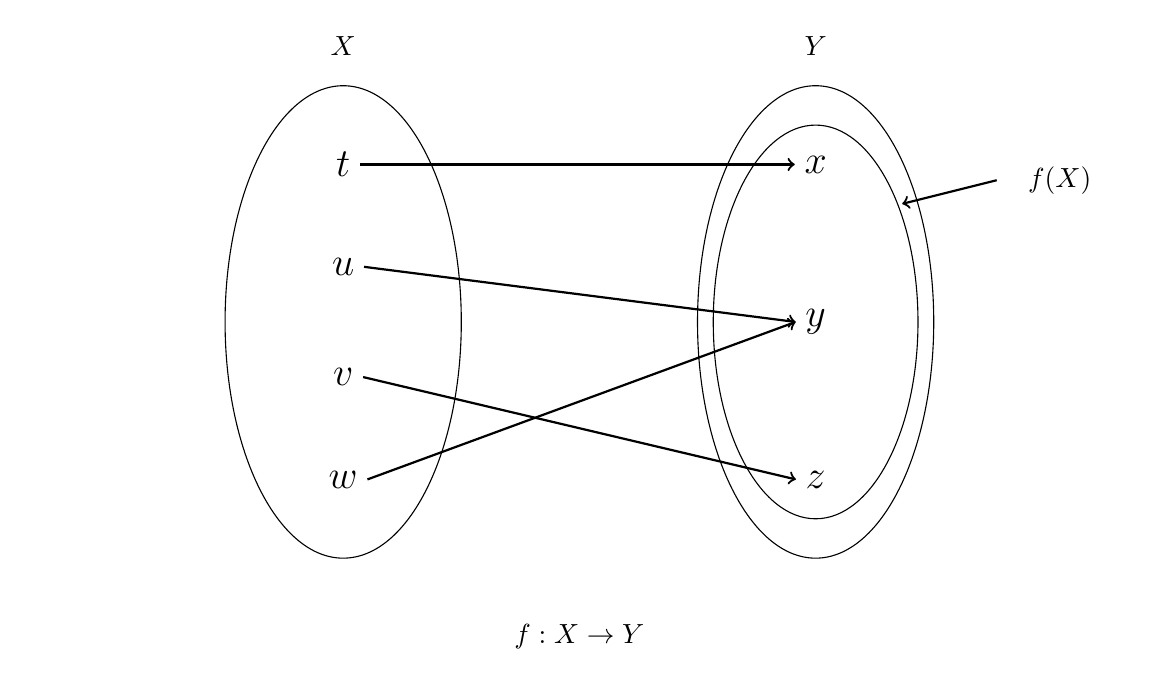
\begin{tikzpicture}
			\filldraw[white] (-7,-3) rectangle (7,3);

			\draw (-3,0) ellipse (1.5 and 3) node[yshift=3.5cm] {$X$};

			\draw (3,0) ellipse (1.5 and 3) node[yshift=3.5cm] {$Y$};
			\draw (3,0) ellipse (1.3 and 2.5);
			\draw[thick, ->] (5.3,1.8) node[xshift=.8cm] {$f(X)$} -- (4.1,1.5);

			\node (t) at (-3,2) {\Large$t$};
			\node (u) at (-3,.7) {\Large$u$};
			\node (v) at (-3,-.7) {\Large$v$};
			\node (w) at (-3,-2) {\Large$w$};

			\node (x) at (3,2) {\Large$x$};
			\node (y) at (3,0) {\Large$y$};
			\node (z) at (3,-2) {\Large$z$};

			\draw[thick,->] (t.east) -- (x.west);
			\draw[thick,->] (u.east) -- (y.west);
			\draw[thick,->] (v.east) -- (z.west);
			\draw[thick,->] (w.east) -- (y.west);

			\draw (0,-4) node {$f:X\to Y$};
	\end{tikzpicture}}
	\caption{}
	\label{fig:sur}
\end{figure}

Then, when you put these together, the resulting function is a bijection as illustrated in \cref{fig:bijection}.

\begin{prop}
	Let $f:X \to Y$ be one-to-one.
	Then $f^{-1}(f(U)) = U$ for some $U \subseteq X$
\end{prop}
\begin{proof}
	Suppose $x\in f^{-1}(f(U))$, then there exists some $y\in f(U)$ such that $f(x)=y$.
	Since $y\in f(U)$, there exists some $x'\in U$ such that $f(x')=y$.
	Thus, $f(x)=f(x')$ whereby the definition of one-to-one, we have $x=x'$ implying $x \in U$; thus we obtain $f^{-1}(f(U)) \subseteq U$.

	By \cref{prop:preimgimg}, we have $U \subseteq f^{-1}(f(U))$, thus we conclude with $f^{-1}(f(U)) = U$ thereby completing the proof.
\end{proof}

\begin{prop} \label{prop:sur-img-preimg}
	Let $f:X \to Y$ be onto $Y$.
	Then $f(f^{-1}(V)) = V$ for some $V \subseteq Y$
\end{prop}
\begin{proof}
	See \cref{exer:sur-img-preimg}.
\end{proof}

\begin{prop} \label{prop:injection-fiber-single}
	A function $f:X \to Y$ is one-to-one if and only if its nonempty fibers are singletons.
\end{prop}
\begin{proof}
	For the forwards direction, suppose $f$ is one-to-one.
	For any $y\in Y$ such that $f^{-1}(y)\neq\varnothing$, choose any $x,x'\in f^{-1}(y)$, then we have $f(x)=f(x')=y$.
	Since $f$ is one-to-one, $x=x'$; thus $f^{-1}(y)$ is a singleton.

	For the backwards direction, suppose all non-empty fibers of $f$ are nonempty.
	Then suppose $f(x)=f(x')$.
	By definition $f^{-1}(f(x))$ is nonempty and contains $x$ and $x'$.
	Since nonempty fibers are singletons, we require $x=x'$ thus proving $f$ is one-to-one.
\end{proof}

\begin{prop} \label{prop:sur-full-image}
	A function $f: \to Y$ is onto $Y$ if and only if the range of $f$ is $Y$.
\end{prop}
\begin{proof}
	Immediate by comparing the definition of range and an onto function.
\end{proof}


\begin{figure}
\centering
\resizebox{0.7\linewidth}{!}{
	\begin{tikzpicture}
		\filldraw[white] (-7,-3) rectangle (7,3);

		\draw (-3,0) ellipse (1.5 and 3) node[yshift=3.5cm] {$X$};

		\draw (3,0) ellipse (1.5 and 3) node[yshift=3.5cm] {$Y$};
		\draw (3,0) ellipse (1.3 and 2.5);
		\draw[thick, ->] (5.3,1.8) node[xshift=.8cm] {$f(X)$} -- (4.1,1.5);

		\node (u) at (-3,2) {\Large$u$};
		\node (v) at (-3,0) {\Large$v$};
		\node (w) at (-3,-2) {\Large$w$};

		\node (x) at (3,2) {\Large$x$};
		\node (y) at (3,0) {\Large$y$};
		\node (z) at (3,-2) {\Large$z$};

		\draw[thick,->] (u.east) -- (y.west);
		\draw[thick,->] (v.east) -- (z.west);
		\draw[thick,->] (w.east) -- (x.west);

		\draw (0,-4) node {$f:X\to Y$};
	\end{tikzpicture}}
	\caption{}
	\label{fig:bijection}
\end{figure}

\begin{prop} \label{prop:comp-in-sur-bi}
	Let $f:X \to Y$ and $g: Y \to Z$ be functions, then the following hold:
	\begin{enumerate}
		\item If $f$ and $g$ are one-to-one, then $g\circ f$ is one-to-one,
		\item if $f$ and $g$ are onto, then $g\circ f$ is onto,
		\item if $f$ and $g$ are bijective, then $f\circ g$ is bijective.
	\end{enumerate}
\end{prop}
\begin{proof}
	See \cref{exer:comp-in-sur-bi}.
\end{proof}

With this newfound vocabulary, we are one step closer to talking about inverses, but before we do, we must discuss function composition.
When we compose functions, we take the output from one function and put it into another.
Because of some properties of this operation resemble multiplication, the symbol we often use for composition often looks like multiplication.\footnote{
	If you ever take linear algebra, function composition distributes on addition very similarly to how multiplication does.
	It also has an interesting connection to matrix multiplication, which could be a source of motivation for the symbol.}

\begin{define}
	Define $f:Y\to Z$ and $g:X\to Y$. The composition of $f$ and $g$, notated as $f\circ g$ is a function $f\circ g:X\to Z$ such that $(f\circ g)(x)=f(g(x))$.
\end{define}

An important property that's useful later is that functional composition is associative, or $f\circ (g\circ h)=(f\circ g) \circ h$. The proof is straightforward, thus left for the reader.
Composition is also illustrated in \cref{fig:comp}.

\begin{figure}
\centering
\resizebox{0.8\linewidth}{!}{
	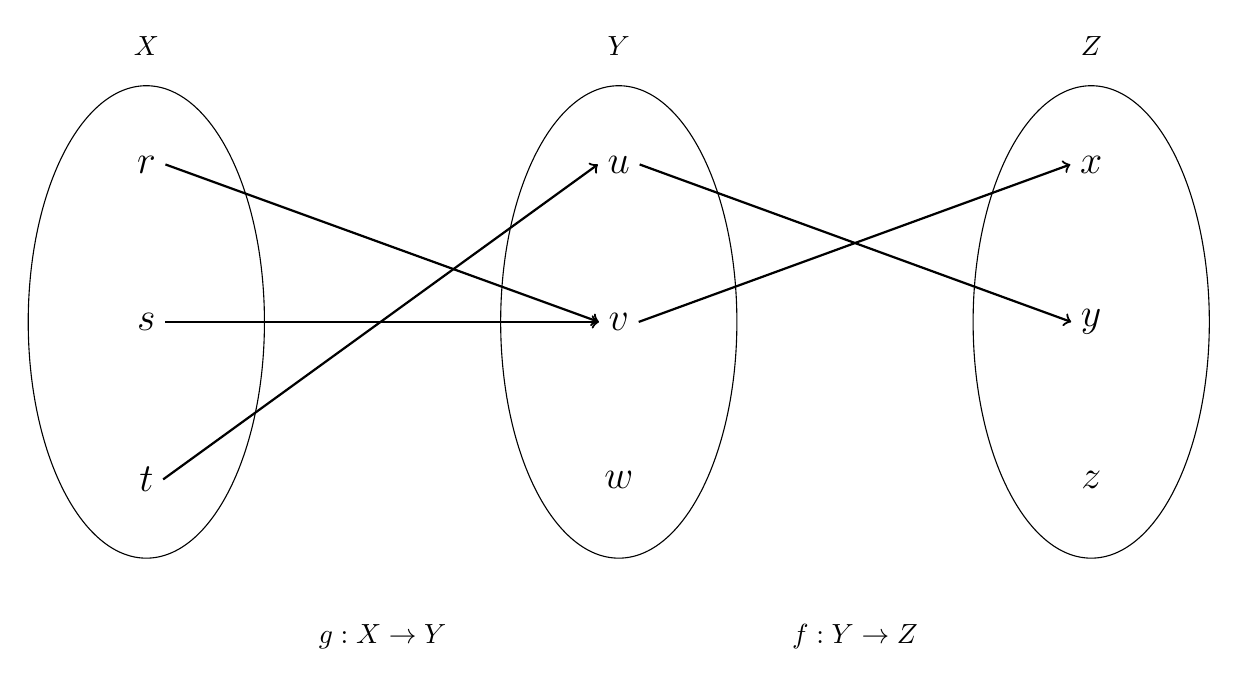
\begin{tikzpicture}
		\draw (-3,0) ellipse (1.5 and 3) node[yshift=3.5cm] {$X$};

		\draw (3,0) ellipse (1.5 and 3) node[yshift=3.5cm] {$Y$};

		\draw (9,0) ellipse (1.5 and 3) node[yshift=3.5cm] {$Z$};

		\node (r) at (-3,2) {\Large$r$};
		\node (s) at (-3,0) {\Large$s$};
		\node (t) at (-3,-2) {\Large$t$};

		\node (u) at (3,2) {\Large$u$};
		\node (v) at (3,0) {\Large$v$};
		\node (w) at (3,-2) {\Large$w$};

		\node (x) at (9,2) {\Large$x$};
		\node (y) at (9,0) {\Large$y$};
		\node (z) at (9,-2) {\Large$z$};

		\draw[thick,->] (r.east) -- (v.west);
		\draw[thick,->] (s.east) -- (v.west);
		\draw[thick,->] (t.east) -- (u.west);

		\draw[thick,->] (u.east) -- (y.west);
		\draw[thick,->] (v.east) -- (x.west);

		\draw (0,-4) node {$g:X\to Y$};
		\draw (6,-4) node {$f:Y\to Z$};
	\end{tikzpicture}}
	\caption{}
	\label{fig:comp}
\end{figure}

\begin{define} \label{def:left}
	Let $f:X\to Y$ be a function. If $g: Y\to X$ is a function such that $g\circ f=\id_X$, then $g$ is the retraction (left inverse) of $f$.
\end{define}

We take $\id_X$ in definition \eqref{def:left} as the following:

\begin{define}
	For any set $X$, let $\id_X:X \to X$ denote the \textit{identity} function on $X$ defined by $\id_X(x)=x$, for any element $x \in X$.\footnotemark
\end{define}
\footnotetext{Notice any composition with the identity function results in the same function (e.g., $f\circ \id_X=\id_Y\circ f=f$).}

\begin{define}
	Let $f:X\to Y$ be a function. If $g: Y\to X$ is a function such that $f\circ g=\id_Y$, then $g$ is the section (right inverse) of $f$.
\end{define}

An example of a retraction is illustrated in \cref{fig:left}.
Likewise, an example of a section is illustrated in \cref{fig:right}.

\begin{figure}
\centering
\resizebox{0.8\linewidth}{!}{
	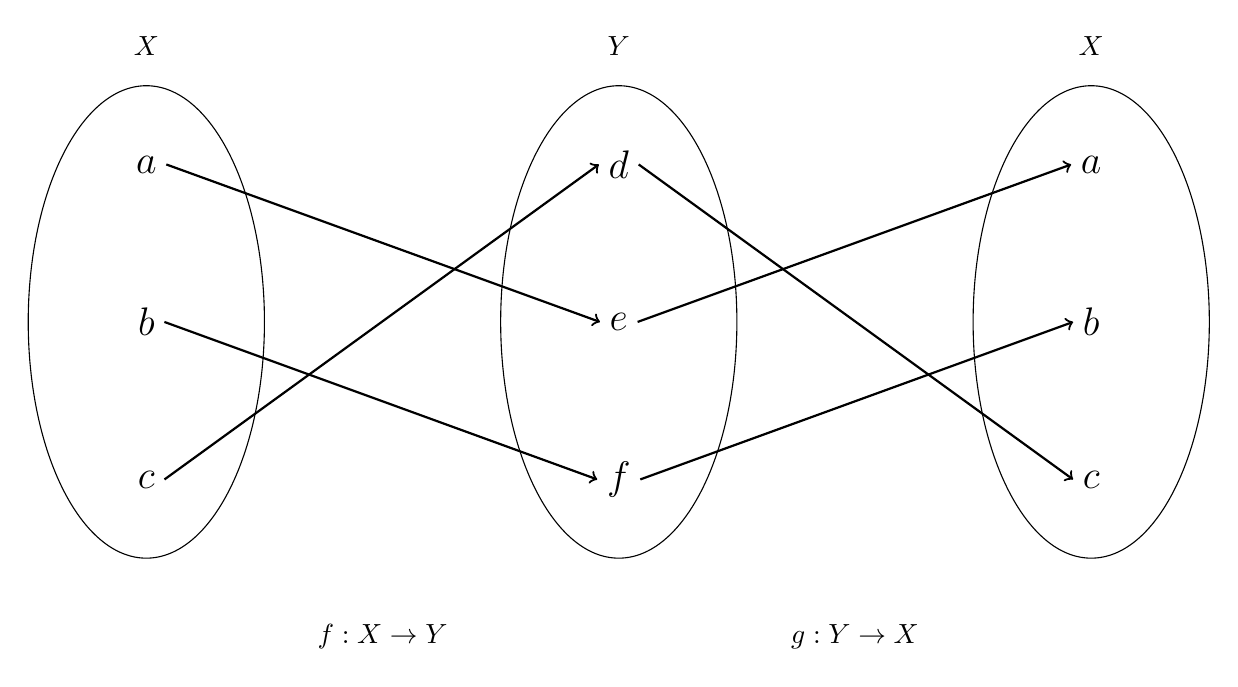
\begin{tikzpicture}
		\draw (-3,0) ellipse (1.5 and 3) node[yshift=3.5cm] {$X$};

		\draw (3,0) ellipse (1.5 and 3) node[yshift=3.5cm] {$Y$};

		\draw (9,0) ellipse (1.5 and 3) node[yshift=3.5cm] {$X$};

		\node (a) at (-3,2) {\Large$a$};
		\node (b) at (-3,0) {\Large$b$};
		\node (c) at (-3,-2) {\Large$c$};

		\node (d) at (3,2) {\Large$d$};
		\node (e) at (3,0) {\Large$e$};
		\node (f) at (3,-2) {\Large$f$};

		\node (g) at (9,2) {\Large$a$};
		\node (h) at (9,0) {\Large$b$};
		\node (i) at (9,-2) {\Large$c$};

		\draw[thick,->] (a.east) -- (e.west);
		\draw[thick,->] (b.east) -- (f.west);
		\draw[thick,->] (c.east) -- (d.west);

		\draw[thick,->] (e.east) -- (g.west);
		\draw[thick,->] (f.east) -- (h.west);
		\draw[thick,->] (d.east) -- (i.west);

		\draw (0,-4) node {$f:X\to Y$};
		\draw (6,-4) node {$g:Y\to X$};
	\end{tikzpicture}}
	\caption{}
	\label{fig:left}
\end{figure}

\begin{figure}
\centering
\resizebox{0.8\linewidth}{!}{
	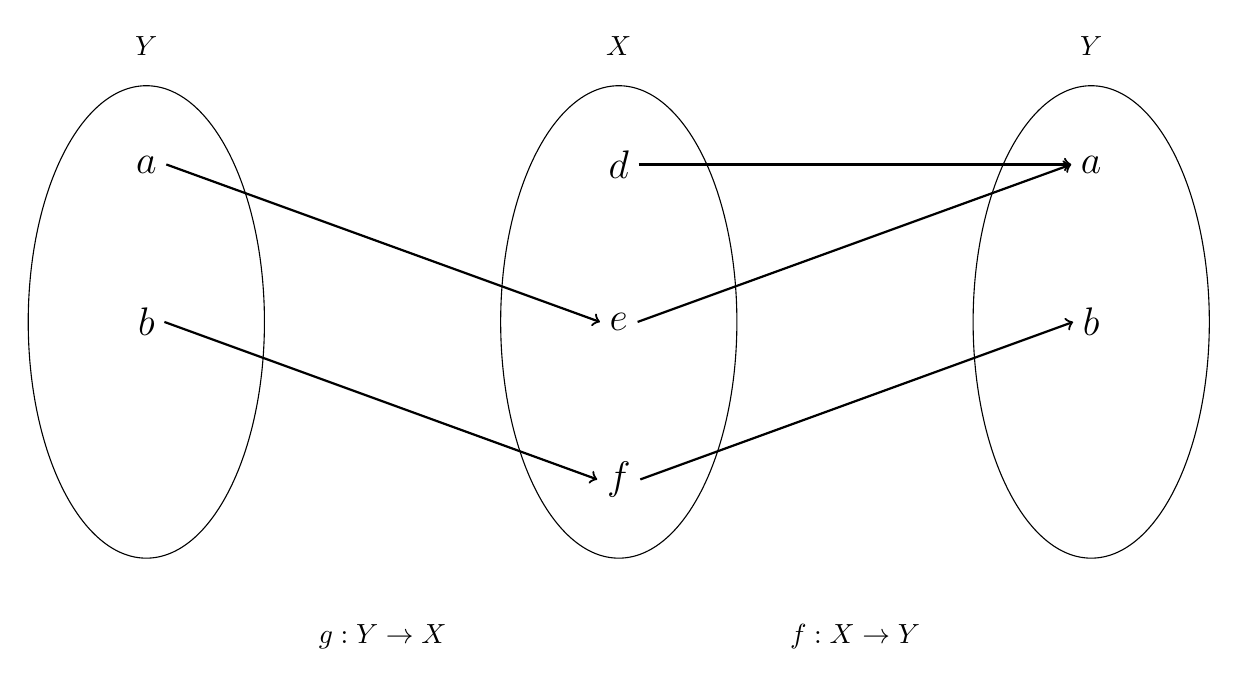
\begin{tikzpicture}
		\draw (-3,0) ellipse (1.5 and 3) node[yshift=3.5cm] {$Y$};

		\draw (3,0) ellipse (1.5 and 3) node[yshift=3.5cm] {$X$};

		\draw (9,0) ellipse (1.5 and 3) node[yshift=3.5cm] {$Y$};

		\node (a) at (-3,2) {\Large$a$};
		\node (b) at (-3,0) {\Large$b$};

		\node (d) at (3,2) {\Large$d$};
		\node (e) at (3,0) {\Large$e$};
		\node (f) at (3,-2) {\Large$f$};

		\node (g) at (9,2) {\Large$a$};
		\node (h) at (9,0) {\Large$b$};

		\draw[thick,->] (a.east) -- (e.west);
		\draw[thick,->] (b.east) -- (f.west);


		\draw[thick,->] (e.east) -- (g.west);
		\draw[thick,->] (f.east) -- (h.west);
		\draw[thick,->] (d.east) -- (g.west);

		\draw (0,-4) node {$g:Y\to X$};
		\draw (6,-4) node {$f:X\to Y$};
	\end{tikzpicture}}
	\caption{}
	\label{fig:right}
\end{figure}

To understand these concepts more, let's prove some basic properties of these inverse.

\begin{theorem} \label{thm:left}
	$f:X \to Y$ is one-to-one with $X\neq\varnothing$ if an only if $f$ has a retraction.
\end{theorem}
\begin{proof}
	For the forward direction, suppose $f$ is one-to-one and $X \neq \varnothing$.
	We have some $x_0 \in X$ since $X$ is nonempty and nonempty fibers are singletons by \cref{prop:injection-fiber-single}.
	Then construct $g: Y \to X$ by
	\begin{equation}
		g(y):=
		\begin{cases}
			f^{-1}(y)	\quad &\text{if } f^{-1}(y) \neq \varnothing \\
			x_0, 		\quad &\text{if} f^{-1}(y) = \varnothing
		\end{cases}\footnotemark
	\end{equation}
	and one can check $g$ indeed satisfies the criteria to be a function as specified in \cref{def:function}.
	By computation, we have
	\begin{equation}
		(g\circ f)(x)=g(f(x))=x
	\end{equation}
	thus $g$ is indeed the retraction of $f$ as required.
	\footnotetext{Small abuse of notation here: $f^{-1}(y)$ refers to the element contained in the one-point-set.}

	For any $x_1 x_2\in X$ such that $f(x_1)=f(x_2)$, let $g:Y\to X$ be the left inverse of $f$. Therefore, by the definition of the function, we have
	\begin{equation}
		g(f(x_1))=g(f(x_2)).
	\end{equation}
	But since $g\circ f=I_x$, we deduce $x_1=x_2$
	hence $f$ is one-to-one.
\end{proof}

\begin{theorem} \label{thm:right}
The function $f:X \to Y$ is surjective if and only if $f$ has a section.\footnotemark
\end{theorem}
\begin{proof}
	For the forward direction see \cref{prop:aoc-sections}.
	%TODO: add prop

	For the backwards direction, suppose $f$ has a section $g$. Then $f \circ g = id_Y$.
	We have
	\begin{equation}
		f(g(Y))=\id_Y(Y)=Y.
	\end{equation}
	Since $g(Y) \subseteq X$, $f(g(Y) \subseteq f(X)$, we have $Y \subseteq f(X)$.
	Therefore, $f(X)=Y$, since $f(X) \subseteq Y$ by definition.
	By \cref{prop:sur-full-image}, $f$ is surjective.
\end{proof}
\footnotetext{
	Note we don't need the nonempty criteria on $X$ since if $X$ is empty, $f$ can't be surjective. See \cref{exer:empty-surjection}
}

\begin{define}
	Let $f:X \to Y$ be a function. Then $f^{-1}:Y \to X$ is the \textit{two-sided inverse} of $f$ if and only if $f \circ f^{-1} = \id_Y$ and $f^{-1}\circ f = \id_X$.
\end{define}

Form here on out, the word \textit{inverse} is defined to mean the \textit{two-sided inverse} unless otherwise specified.

\begin{theorem} \label{thm:bi}
	A function $f:X \to Y$ has an inverse if and only if $f:X \to Y$ is a bijection.
\end{theorem}
\begin{proof}
	The forward direction is immediate by \cref{thm:left} and \cref{thm:right}, since the inverse is also the retraction and section of $f$.

	The existence the inverse on each side is given by \cref{thm:left} and \cref{thm:right}.
	Then \cref{exer:bi-unique} shows these functions are the same, thus completing the proof.
\end{proof}

Working with one-to-one, onto, or bijective functions can be incredibly useful in math, but functions in general can't be characterized by any of these adjectives.
Thus, let's introduce some function operations to facilitate with this.

\begin{define}
	Let $f:X\to Y$. Then we define $f| _A: A\to Y$, where
	$f|_A(a):=f(a)$, to be the \textbf{restriction of $f$ on $A$}
\end{define}
\begin{define}
	Let $f:X\to Y$. Then if $f|^B:X\to B$, where $f|^B(x):=f(x)$, is a well-defined function, then we call $f|^B$ the \textbf{corestriction of $f$ on $B$}.
\end{define}

We note that whilst the restriction of a function always exists, so long as $A$ is non-empty, the corestriction might not always be a well-defined function.
So, let's examine what guarantees the existence of $f|^B$.

\begin{prop}
	Suppose $f:X\to Y$.
	$f|^B$ is a function if and only if $f(X)\subseteq B$.
	\label{prop:well-def-core}
\end{prop}
\begin{proof}
	Suppose $f|^B$ is a function and let $y\in f(X)$.
	Then, by the definition of an image, there exists $x\in X$ such that $f(x)=y$. Then, by the definition of $f|^B$,
	$$f(x)=f|^B=y.$$
	Since $f|^B$ is a function, we have $y\in B$ implying $f(X)\subseteq B$.

	Then suppose $f(X)\subseteq B$. Then, we prove $f|^B$ is a function by checking with \cref{def:function}.
	First, we check that $f|^B$ satisfies (1). This is done by noticing that for every $x\in X$, we have
	$$f|^B(x)=f(x)\in f(X)\subseteq B,$$
	hence $f|^B$ satisfies (1).

	To show $f|^B$ satisfies (2), we notice if $x_1,x_1\in X$$x_1=x_2$, we have
	$$f|^B(x_1):=f(x_1)=f|^B(x_2):=f(x_2).$$
	Since $f$ is a well-defined function, we have $x_1=x_2$.
\end{proof}

By observing the definition of the corestriction and condition that a function is onto, we have the following theorem:

\begin{prop} \label{prop:co-onto}
	For any $f:X\to Y$, if $B\supseteq f(X)$, then $f|^B$ is a onto $B$.
\end{prop}
\begin{proof}
	Let $B=f(X)$. By \cref{prop:well-def-core}, $f$ satyfies the condition to be a function.
	Observe \cref{prop:sur-full-image}, $f$ is clearly onto $B$.
\end{proof}

The proposition makes the following result immediate:

\begin{cor}
	Let $f:X \to Y$ be one-to-one, then $f$ corestricts to a bijection.
\end{cor}

Similarly, we can always restrict a function to be one-to-one.

\begin{prop} \label{prop:re-one}
	For any $f:X\to Y$, there exists $f|_A$, $A\subseteq X$	where $f|_A$ is one-to-one.
\end{prop}
\begin{proof}
	By \cref{prop:co-onto}, we have $f(X)$ such that $f|^{f(X)}$ such that the corestriction is surjective.
	Thus $f|^{f(X)}$ admits a section $g:f(X) \to X$ such that $f|^{f(X)} \circ g = \id_{f(X)}$ by \cref{thm:right}.
	Take $A:=g(f(X))$, we show this makes $f$ one-to-one.

	Suppose for $x_1, x_2\in A$, suppose $f(x_1)=f(x_2)$.
	By definition, $x_1=g(y_1)$ and $x_2=g(y_2)$ for some $y_1,y_2 \in f(X)$.
	Since we have
	\begin{align}
		&f(x_1)=f|^{f(X)}(x_1)=f|^{f(X)}(g(y_1))=\id_Y(y_1)=y_1 \\
		&f(x_2)=f|^{f(X)}(x_2)=f|^{f(X)}(g(y_2))=\id_Y(y_2)=y_2
	\end{align}
	Therefore, by $f(x_1)=f(x_2)$, we have $y_1=y_2$.
	Since $g$ is well-defined, we  require $x_1=x_2$ thus proving proposition.
\end{proof}

Since sections need not be unique for a function, the restriction here is not unique,
In general, for an arbitrary function the restriction down to an injection may not be of much use, but in cases where we have chosen a particular section, this theorem provides an algorithm for producing an injection compatible with the given section.
We should also note the restriction here promotes any section to a two-sided inverse as the corestriction of the restriction on its image gives a bijection.
It follows that the section is the unique inverse on the resulting function.

%TODO: Add examples of inverses and things.

\begin{prop} \label{prop:prod-func-eq}
	For any set $X$, there exists a bijection of the form $\prod_{x \in X} Y \to Y^X$.
\end{prop}
\begin{proof}
	Define $\phi: \prod_{x \in X} Y \to Y^X$ such that $\phi((c_i)_{i\in X})(x)=c_x$.
	One can easily check that this is a well-defined function.

	Then suppose $\phi((c_x)_{x\in X})(x)=\phi((c_x)_{x \in X})(x)$.
	The function definition implies for each $x\in X$, $c_x = c'_x$.
	Therefore $(c_x)_{x \in X} = (c_x')_{x \in X}$ implying $\phi$ is injective.

	For surjectivity, for each $f(x) \in Y^X$, construct the tuple $(f(x))_{x \in X}$.
	Then by definition, this tuple maps to $f$ under $\phi$.
	Therefore, $\phi$ is the bijection as desired.
\end{proof}

We can extend \cref{prop:prod-func-eq} to arbitrary products by replacing $Y^X$ with the subset
\begin{equation}
	\{f \in C^I \mid f(i) \in C_I\}
\end{equation}
where $C$ is the union of the collection $\mathcal C$ and $I$ is an indexing on $\mathcal C$ (see exercise \cref{exer:prod-func-eq}).

If back to the definition of a bijection, we can think of them as pairings of elements between two sets.
For this reason, we can think of a bijection as simply a relabeling map which identifies every object in a set with a new representation in another set and vise versa.
Think of bijections in this way, what \cref{prop:prod-func-eq} tells us is that the set of functions and the set of tuples are the same set up to some relabeling.
This idea of objects being the same up to some relabeling is very common and we often denote these relations as \textit{isomorphisms}.\footnote{We often reserve the term \textit{isomorphism} to situations where there is something other than the set structure being preserved. We will touch on this later when we construct more complicated mathematical objects.}

For two sets under bijection, while these two sets may not be equivalent as sets (i.e. they don't contain precisly the same elements), since the specific interpretation of each element in a set doesn't really matter for most applications (and for much of math for that matter), bijective equivilence is as strong of an conclusion as one will ever need in set theory.\footnote{For a set with nothing else defined, generally, the only property that we are interested in preserving is the \textit{number of elements} a set contains, which bijections do a perfectly fine job of preserving.}
For example, the set of natural numbers, whilst traditionally represented by Arabic numerals, would functionally still be the natural numbers even if we replaced every symbol with random Egyptian hieroglyphics, just so long as the interactions between the symbols are retained to some degree (like the ordering properties, or the way two symbols add or multiply).
As we get further in math, we find that we generally stop giving individual symbols in set specific interpretations and only provide a definition of how these symbols interact.
